% !TEX root = ../main.tex

\section{Опис руху}
Вважаємо, що гра відбувається у \emph{фазовому просторі} $\E$ --- деякій області в $\R^n$ та на її межі.
Рух точки $x = \l(x_1, x_2, ..., x_n \r)$ у фазовому просторі описується системою диференціальних рівнянь
\begin{gather}\label{eq_1}
    \begin{cases}
        \d{x_1}(t) = f_1(x_1(t), ..., x_n(t), u_1(x, t), ..., u_P(x, t), v_1(x, t), ..., w_E(x, t)) \\
        \d{x_2}(t) = f_2(x_1(t), ..., x_n(t), u_1(x, t), ..., u_P(x, t), v_1(x, t), ..., w_E(x, t)) \\
        \dots \\
        \d{x_n}(t) = f_n(x_1(t), ..., x_n(t), u_1(x, t), ..., u_P(x, t), v_1(x, t), ..., w_E(x, t)) \\
        x_1(0) = x_1^0, x_2(0) = x_2^0, ..., x_n(0) = x_n^0
    \end{cases}
\end{gather}
або, коротше,
\begin{gather}\label{eq_2}
    \begin{cases}
        \d{x}(t) = {f}(x(t), u(x, t), v(x, t)) \\
        x(0) = x_0
    \end{cases}
\end{gather}
Ці рівняння називаються \emph{рівняннями руху}. Функції $f_j$ є заданими та вважаються достатньо гладкими.
Функції від часу $u$ та $v$ називаються \emph{керуванням} та змінюються, відповідно, першим та другим гравцем, яких
позначатимемо $P$ та $E$. Ці позначення не є випадковими: вони походять від слів pursuer (переслідувач) та evader (утікач), оскільки
саме такі задачі переслідування-втечі дали початок розвитку теорії диференціальних ігор.

Фазові координати $x_1, ..., x_n$ описують стан гри в тому сенсі, що якщо зупинити гру в будь-який момент часу, зафіксувати значення фазових координат
та почати нову гру з цієї зафіксованої точки фазового простору, то її хід буде таким самим, як у початкової гри після моменту зупинки. Зокрема,
значення $x_0$ фазових координат на початку гри, власне, є всім необхідним набором початкових даних, тому, навіть при однакових $f_j$ та керуваннях,
за різних початкових умов отримуватимемо, взагалі кажучи, різні <<партії>> гри.
\begin{example}
    Якщо позначити через $(x_P, y_P)$ координати гравця $P$, через $(x_E, y_E)$ --- гравця $E$, через $w_P$ та $w_E$ їх сталі швидкості руху, 
    а керування напрямком швидкості через $u(t)$ та $v(t)$ відповідно, то отримаємо такі рівняння руху:
    \begin{gather*}
        \begin{cases}
            \d{x_P}(t) = w_P \cos u(t) \\
            \d{y_P}(t) = w_P \sin u(t) \\
            \d{x_E}(t) = w_E \cos v(t) \\
            \d{y_E}(t) = w_E \sin v(t) \\
            (x_P(0), y_P(0)) = (x_P^0, y_P^0) \\
            (x_E(0), y_E(0)) = (x_E^0, y_E^0)
        \end{cases}
    \end{gather*}    
    Такий рух називається <<переслідуванням на площині з простим рухом гравців>>.
\end{example}
\begin{example}[гра <<водій-вбивця>>, \cite{1}]
    В цьому випадку гра також відбувається на площині. Переслідувач $P$ рухається зі сталою швидкістю $w_P$, радіус кривини його траєкторії обмежений
    заданою величиною $R$. Керування $P$ --- це вибір значення кривини в кожний момент часу. Рух утікача $E$ простий: швидкість $w_E$ фіксована,
    керуванням є вибір напрямку швидкості $v(t)$. $E$ в деякому сенсі є більш маневреним, ніж $P$.
    Фазовими координатами в цій грі є пари $x_P, y_P$ і $x_E, y_E$ для опису положення $P$ та $E$ відповідно, та $\theta$ --- напрямок руху $P$.
    \begin{center}
        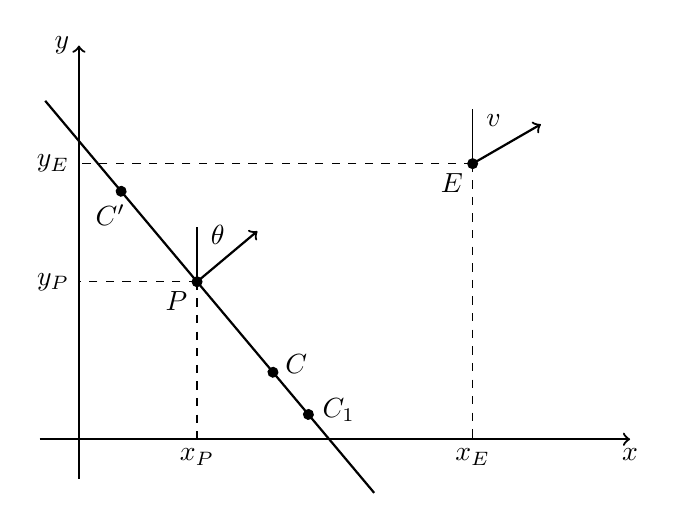
\begin{tikzpicture}
            \draw [->, thick] (-0.5, 0) -- (7, 0);
            \draw [->, thick] (0, -0.5) -- (0, 5);
            \node [below] at (7, 0) {$x$};
            \node [left] at (0, 5) {$y$};
            % P
            \fill (1.5, 2) circle [radius=2pt];
            \node [below left] at (1.5, 2) {$P$};
            \draw [dashed] (1.5, 2) -- (1.5, 0);
            \draw [dashed] (1.5, 2) -- (0, 2);
            \node [below] at (1.5, 0) {$x_P$};
            \node [left] at (0, 2) {$y_P$};
            \draw (1.5, 2) -- (1.5, 2.7);
            \draw [thick, ->, rotate around={-50:(1.5, 2)}] (1.5, 2) -- (1.5, 3);
            \centerarc[] (1.5, 2) (40:90:0.5);
            \node [above right] at (1.5+0.05, 2+0.35) {$\theta$};
            \draw [thick, rotate around={-50:(1.5, 2)}] (1.5-3, 2) -- (1.5+3.5, 2);
            \fill [rotate around={-50:(1.5, 2)}] (1.5-1.5, 2) circle [radius=2pt];
            \node [below] at (0.4, 3.1) {$C'$};
            \fill [rotate around={-50:(1.5, 2)}] (1.5+1.5, 2) circle [radius=2pt];
            \node [above] at (2.76, 0.71) {$C$};
            \fill [rotate around={-50:(1.5, 2)}] (1.5+2.2, 2) circle [radius=2pt];
            \node [above] at (3.3, 0.1) {$C_1$};
            % E
            \fill (5, 3.5) circle [radius=2pt];
            \node [below left] at (5, 3.5) {$E$};
            \draw [dashed] (5, 3.5) -- (5, 0);
            \draw [dashed] (5, 3.5) -- (0, 3.5);
            \node [below] at (5, 0) {$x_E$};
            \node [left] at (0, 3.5) {$y_E$};
            \draw (5, 3.5) -- (5, 4.2);
            \draw [thick, ->, rotate around={-60:(5, 3.5)}] (5, 3.5) -- (5, 4.5);
            \centerarc[] (5, 3.5) (30:90:0.5);
            \node [above right] at (5+0.05, 3.5+0.35) {$v$};
        \end{tikzpicture}
    \end{center}
    Керування $E$ --- це вибір кута швидкості $v$. Керування $P$ записати дещо складніше. Проведемо через точку $(x_P, y_P)$
    пряму $C' P C$, $|C' P| = |P C| = R$, перпендикулярну до вектору швидкості $P$. $P$ обирає миттєвий центр кривини своєї траєкторії у довільній точці $C_1$ цієї
    прямої, що лежить за межами відрізку $C' C$ (оскільки радіус кривини обмежений). Керування $u(t)$ будемо вважати рівним за модулем
    $R / |P C_1|$, додатним для точок $C_1$, що знаходяться правіше від $P$, та від'ємним для тих, що знаходяться лівіше. Остаточно, маємо такі рівняння руху:
    \begin{gather*}
        \begin{cases}
            \d{x_P}(t) = w_P \sin \theta(t) \\
            \d{y_P}(t) = w_P \cos \theta(t) \\
            \d{x_E}(t) = w_E \sin v(t) \\
            \d{y_E}(t) = w_E \cos v(t) \\
            \d{\theta}(t) = \frac{w_P}{R} u(t), \; u(t) \in [-1; 1]
        \end{cases}
    \end{gather*}
\end{example}

\section{Виграші та стратегії гравців}
Мета диференціальної гри визначається виграшем, який деяким чином
залежить від траєкторій, що пройшли гравці до завершення гри. Позначимо ці траєкторії як функції від часу
як $x(t)$ та $y(t)$. Зауважимо, що диференціальні ігри є \emph{антагоністичними} (або ж, \emph{іграми з нульовою сумою}).

Якщо гра триває деякий заздалегідь визначений час $T$, то виграш гравця $E$ визначається
як $H(x(t), y(T))$, де $H : \R^n \times \R^n \to \R$ --- деяка функція (нагадаємо, що розмірність $\E$ --- $n$). Наприклад, якщо
$$H(x(T), y(T)) = \norm{x(T) - y(T)}$$ то гра описуватиме процес переслідування, в якому
метою гравця $E$ є відхилення від гравця $P$ на момент кінця гри на максимально можливу відстань.
В цьому випадку антагоністичність означає, що метою $P$ є, навпаки, максимальне зближення з $E$ на момент $t=T$. 
Також, можна в якості $H$ використовувати $$H(x(T), y(T)) = \underset{0 \leq t \leq T}{\min} \norm{x(t) - y(t)}$$
Це означатиме, що гравцю $E$ потрібно не просто віддалитися від $P$ в останній момент гри,
а й триматися якнайдалі від $P$ протягом усього часу гри. Це буде так званий \emph{мінімальний виграш}.

Гра також може завершуватися, коли обидва гравці потраплять до деякої підмножини $\T \subset \E$.
Тоді в якості виграшу гравця $E$ можна покласти
$$t_* = \min \l\{ t \geq 0 : (x(t), y(t)) \in \T\r\}$$
$t_*$ --- перший момент потрапляння гравців до $\T$ (або <<захоплення гравцем $P$>>).
Такий виграш називається \emph{термінальним виграшем}. Якщо для всіх $t \geq 0$ вони ніколи не потрапляють до $\T$,
то виграш гравця $E$ дорівнює $+\infty$. Наприклад, якщо в якості $\T$ взяти гіперсферу радіуса $l\geq 0$,
то метою гравця $P$ буде якнайшвидше зближення з $E$ на відстань $l$. Можна також поставити задачу пошуку
таких множин початкових умов, за яких $t_*$ гарантовано буде скінченним або нескінченним. 
В такому випадку можна ввести \emph{якісний виграш}, що набуває значень $\pm 1$ в залежності від того,
чи вдалося $E$ уникнути захоплення гравцем $P$.

\begin{example}(\cite{2})
    Розглянемо переслідування на площині з простим рухом, що описується системою
    \begin{gather*}
        \begin{cases}
            \d{x_1} = u_1, \d{x_2} = u_2, \; u_1^2 + u_2^2 \leq \alpha^2 \\
            \d{y_1} = v_1, \d{y_2} = v_2, \; v_1^2 + v_2^2 \leq \beta^2 \\
            x_1(0) = x_1^0, x_2(0) = x_2^0, y_1(0) = y_1^0, y_2(0) = y_2^0
        \end{cases}
    \end{gather*}
    Тут $P(t) = (x_1, x_2)$ --- координати гравця $P$, $E(t) = (y_1, y_2)$ --- координати гравця $E$.
    $u_1, u_2$ та $v_1, v_2$ --- їх керування відповідно, причому з умови швидкості руху (зміни координат гравців) обмежені
    максимальними значеннями $\alpha$ та $\beta$. Обидва гравці, обираючи керування, змінюють напрямок руху.
    
    Якщо $\alpha > \beta$, то гравець $P$ може гарантувати
    \begin{gather*}
        \forall l \geq 0 : \min \l\{ t \geq 0 : \norm{P(t) - E(t)} \leq l\r\} < +\infty
    \end{gather*}
    тобто, наближення до $E$ на будь-яку відстань за скінченну кількість часу.
    Для цього достатньо рухатися з максимальною швидкістю $\alpha$ в тому ж напрямку, що і $E$.

    Якщо $\alpha \leq \beta$, то в разі $\norm{P(0) - E(0)} > l$ для всіх $l \geq 0$ гравець $E$, рухаючись від $P$ по прямій з максимальною швидкістю,
    зможе уникнути захоплення гравцем $P$.
\end{example}

\begin{definition}
    \emph{Стратегіями} у диференціальній грі є вибір керувань $u$ та $v$ як функцій від часу $t$ та
фазових координат $x$ у системі рівнянь руху (\ref{eq_1}).
\end{definition}
Керування вважаються кусково-гладкими як компроміс між забезпеченням існування розв'язку,
(його може не існувати у класі неперервних функцій) та його єдиності (вона може порушуватися, якщо не вимагати неперервності розв'язку).
Позначатимемо через $\rm P$ та $\rm E$ множини кусково-неперервних стратегій (керувань) гравців $P$ та $E$. 

Надалі для спрощення розглядатимемо не один вектор $x$, а два вектори $x$ та $y$, що відповідатимуть руху кожного з гравців. Тоді
систему (\ref{eq_2}) можна записати як
\begin{gather}\label{eq_3}
    \begin{cases}
        \d{x}(t) = f(x(t), u(x, y, t)) \\
        \d{y}(t) = g(x(t), v(x, y, t)) \\
        x(0) = x_0, y(0) = y_0
    \end{cases}
\end{gather}

\begin{definition}
    Набір $S = \l\{x_0, y_0, u(\cdot), v(\cdot) \r\}$, де $x_0, y_0$ --- початкові умови, а $u \in \rm P$, $v \in \rm E$ --- керування, 
    називається \emph{ситуацією} в диференціальній грі. 
\end{definition}
Якщо розглядати траєкторії, що залежать лише від часу $t$ та накладати на $f$ та $g$ умови
обмеженості та ліпшицевості по $x$ та $y$, тобто
\begin{gather*}
    \norm{f(x_1, u) - f(x_2, u)} \leq \alpha \cdot \norm{x_1 - x_2}, \;
    \norm{g(y_1, v) - g(y_2, v)} \leq \beta \cdot \norm{y_1 - y_2}
\end{gather*}
то за теоремою про існування та єдиність роз'язку задачі Коші, для кожної ситуації $S$ буде існувати єдина пара траєкторій $x(t), y(t)$,
для якої
\begin{gather*}
    \begin{cases}
        \d{x}(t) = f(x(t), u(t)) \\
        \d{y}(t) = g(y(t), v(t)) \\
        x(0) = x_0, y(0) = y_0
    \end{cases}
\end{gather*}

\begin{definition}
    Користуючись означенням ситуації, можна ввести \emph{виграш} в ситуації $S = \l\{x_0, y_0, u(\cdot), v(\cdot) \r\}$
    як функцію $K(x_0, y_0, u(\cdot), v(\cdot))$.
\end{definition}
Приклади виграшів було наведено вище. Траєкторії $x(t)$ та $y(t)$ в них визначаються саме з ситуації $S$. Наведемо строгі означення.
\begin{definition}
        \emph{Термінальний виграш}. Задано деяке число $t>0$ та неперервна по $x$ та $y$ функція $H(x, y)$. Виграш в ситуації $\l\{x_0, y_0, u(\cdot), v(\cdot) \r\}$
        визначається як
        \begin{gather*}
            K(x_0, y_0, u(\cdot), v(\cdot)) = H(x(T), y(T))
        \end{gather*}
        
        \emph{Мінімальний результат}. Задано деяке число $t>0$ та неперервна по $x$ та $y$ функція $H(x, y)$. Виграш в ситуації $\l\{x_0, y_0, u(\cdot), v(\cdot) \r\}$
        визначається як
        \begin{gather*}
            K(x_0, y_0, u(\cdot), v(\cdot)) = \underset{0 \leq t \leq T}{\min} H(x(t), y(t))
        \end{gather*}
        
        \emph{Інтегральний виграш}. Нехай $\T$ --- деяка підмножина $\R^n \times \R^n$, $H(x, y)$ --- неперервна функція. Нехай в ситуації $\l\{x_0, y_0, u(\cdot), v(\cdot) \r\}$
        $t_*$ --- перший момент потрапляння траєкторії $(x(t), y(t))$ на $\T$.
        Тоді
        \begin{gather*}
            K(x_0, y_0, u(\cdot), v(\cdot)) = \intl_0^{t_*} H(x(t), y(t)) dt
        \end{gather*}
        де при $t_* = +\infty$ покладається $K = +\infty$.

        \emph{Якісний виграш}. Нехай $\T$ та $\mathcal{L}$ --- деякі підмножини $\R^n \times \R^n$, а $t_*$ --- перший момент потрапляння траєкторії $(x(t), y(t))$ на $\T$
        в ситуації $\l\{x_0, y_0, u(\cdot), v(\cdot) \r\}$. Тоді
        \begin{gather*}
            K(x_0, y_0, u(\cdot), v(\cdot)) = \begin{cases}
                1, & \text{ якщо } (x(t_*), y(t_*)) \in \mathcal{L} \\
                0, & \text{ якщо } t_* = +\infty \\
                -1, & \text{ якщо } (x(t_*), y(t_*)) \notin \mathcal{L} \\
            \end{cases}
        \end{gather*}
\end{definition}

Нарешті, можна дати означення нормальної форми диференціальної гри.
\begin{definition}
    Нормальною формою диференціальної гри $\Gamma (x_0, y_0)$, заданої на просторі стратегій $\mathrm{P} \times \mathrm{E}$, називається система
    \begin{gather}
        \Gamma (x_0, y_0) = \l<x_0, y_0, \mathrm {P}, \mathrm{E}, K(x_0, y_0, u(\cdot), v(\cdot)) \r>
    \end{gather}
    де $K(x_0, y_0, u(\cdot), v(\cdot))$ --- функція виграшу, визначена будь-який з чотирьох способів вище.
\end{definition}
\begin{remark}
    Кожній парі $(x_0, y_0) \in \R^n \times \R^n$ відповідає своя гра в нормальній формі, тобто, фактично,
    визначається двопараметрична сім'я ігор, що залежать від $(x_0, y_0)$.
\end{remark}
Часто гру називають за функцією виграшу грою з термінальним, інтегральним, якісним виграшем або грою на досягнення мінімального результату.